\lhead[\thepage]{CAPÍTULO \thechapter. VERIFICACIÓN, VALIDACIÓN Y EVALUACIÓN}
\chead[]{}
\rhead[WepSIM: Simulador de un procesador elemental con unidad de control microprogramada\leftmark]{\thepage}
\renewcommand{\headrulewidth}{0.5pt}

\lfoot[]{}
\cfoot[]{}
\rfoot[]{}
\renewcommand{\footrulewidth}{0pt}

%% This is an example first chapter.  You should put chapter/appendix that you
%% write into a separate file, and add a line \include{yourfilename} to
%% main.tex, where `yourfilename.tex' is the name of the chapter/appendix file.
%% You can process specific files by typing their names in at the 
%% \files=
%% prompt when you run the file main.tex through LaTeX.
\chapter{Verificación, validación y evaluación}
\label{ch:verification_validation_and_evaluation}
\markboth{}{VERIFICACIÓN, VALIDACIÓN Y EVALUACIÓN}


Este capítulo detalla la verificación, validación y evaluación del proyecto. En primer lugar, presentamos la verificación y validación del simulador (Sección \ref{sec:verification_and_validation}, \textit{\nameref{sec:verification_and_validation}}), y detallamos una serie de pruebas que nos permitieron verificar que habíamos cumplido todos los requisitos establecidos en el Capítulo  \ref{ch:analysis}(\textit{\nameref{ch:analysis}}). Después de esto, mostramos la validación de los resultados de las simulaciones, demostrando que el simulador realiza simulaciones precisas y realistas.

Para la realización de las simulaciones, hemos tomado la definición de un juego de instrucciones base proporcionado por el coordinador de la asignatura Estructura de Computadores, pudiendo así validar que el funcionamiento del simulador es correcto al obtener los resultados esperados en cada una de las instrucciones y códigos simulados en la herramienta. 

\section{Verificación y validación}
\label{sec:verification_and_validation}

El principal objetivo de esta sección es verificar que todos los requisitos detallados en el Capítulo \ref{ch:analysis} (\textit{\nameref{ch:analysis}}) han sido cumplidos. Además, validamos los resultados obtenidos con WepSIM, comparándolos con los resultados teóricos esperados de la definición del juego de instrucciones de la asignatura Estructura de Computadores y los ejercicios especificados en el libro de la asignatura \cite{perez2015problemas}.


En la Ingeniería del Software, la verificación y validación son los procesos de comprobar que un sistema de software cumple con las especificaciones y que cumple con su propósito. Como se explica en el Capítulo \ref{ch:analysis} (\textit{\nameref{ch:analysis}}), el cliente fija inicialmente los requisitos deseados para el producto final (requisitos del usuario). A partir de ahí, los analistas especifican los requisitos de software (requisitos funcionales y no funcionales). Para verificar que se cumplen los requisitos del proyecto, se necesitan procesos de verificación y validación (ver Figura \ref{fig:verification_validation}).

\vspace{1cm}

\begin{figure}[htb]
 	\centering
 	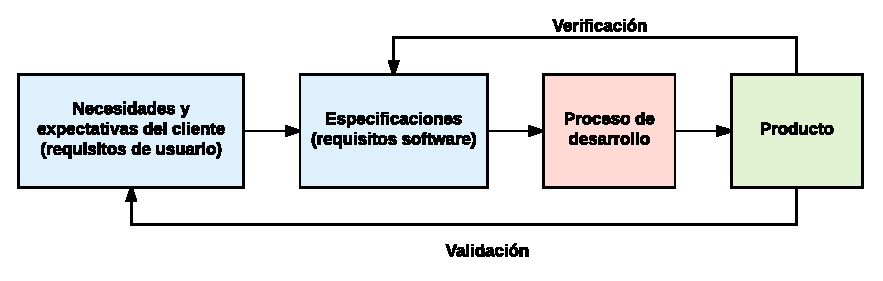
\includegraphics[width=12cm]{figures/verificacion_validacion_diagrama}
 	\caption{Verificación y validación software.}
	\label{fig:verification_validation}
\end{figure}

\vspace{1cm}

\textit{Verificación Software} Es el proceso de evaluación de los productos de trabajo (no el producto final real) de una fase de desarrollo para determinar si cumplen con los requisitos especificados para esa fase (los requisitos de software). \textit{Validación software} es el proceso de evaluación del producto final al final del proceso de desarrollo para determinar si satisface los requisitos especificados por el usuario al inicio del proyecto \cite{verification}.

\subsection{Pruebas de verificación}

Con el fin de realizar las pruebas de verificación, hemos seguido un proceso dinámico durante la fase de desarrollo del software. Con estas pruebas queríamos responder a la pregunta: \emph{``¿Estamos construyendo el producto correctamente?''}. La Tabla \ref{tab:verification_tests} proporciona la plantilla utilizada para los test de verificación. Es necesario tener en cuenta que el formato del atributo ID es VET-XX, donde XX indica el número de test de verificación.
\clearpage

\begin{center}
\begin{table*}[htb]
\centering
\caption{Plantilla de pruebas de verificación.}
\begin{tabular}{@{}p{2.5cm} p{9cm}@{}} 
\toprule
\textbf{ID} 					& Test ID. \\
\midrule
\textbf{Nombre} 				& Nombre del test. \\
\midrule
\textbf{Requisitos} 		& Requisitos de software cumplidos con este test. \\
\midrule
\textbf{Descripción} 		& Descripción del test. \\
\midrule
\textbf{Precondiciones}		& Las condiciones que siempre deben ser verdad antes de realizar el test. \\
\midrule
\textbf{Procedimiento}			& Una secuencia fija, paso a paso, de las actividades realizadas por el test. \\
\midrule
\textbf{Postcondiciones} 		& Las condiciones que siempre deben ser verdaderas justo después de realizar el test. \\
\midrule
\textbf{Evaluación} 			& \textit{OK} o \textit{Error}. \\
\bottomrule
\end{tabular}
\label{tab:verification_tests}
\end{table*}
\end{center}

A continuación, se especifican las pruebas de verificación.

\begin{center}
\begin{table*}[htb]
\centering
\caption{Test de verificación VET-01.}
\begin{tabular}{@{}p{2.5cm} p{13cm}@{}} 
\toprule
\textbf{ID} 					& VET-01. \\
\midrule
\textbf{Nombre} 				& Plataforma. \\
\midrule
\textbf{Requisitos} 		& SR-NF-PL01, SR-NF-PL02\\
\midrule
\textbf{Descripción} 		& Verificar que el software puede ser utilizado en los navegadores especificados en los requisitos. \\
\midrule
\textbf{Precondiciones}		& 1. Utilizar un computador con sistema operativo Ubuntu 16.04 / Windows 10 / MacOS 10.2.5 .\\
							& 2. .Tener instalados los navegadores Microsft Edge 30+, Mozilla Firefox 45+, Google Chrome 50+ o Safari 10+. \\
\midrule
\textbf{Procedimiento}			& 1. Abrir el software en cualquiera de los navegadores web especificados. \\
							& 2. Generar firmware.\\
							& 3. Generar memoria principal.\\
							& 4. Ejecutar simulación.\\
\midrule
\textbf{Postcondiciones} 		&  La simulación ha sido completada satisfactoriamente sin ningún error de ejecución debido a la plataforma .\\
\midrule
\textbf{Evaluación} 			& OK \\
\bottomrule
\end{tabular}
\label{tab:vet01}
\end{table*}
\end{center}

\begin{center}
\begin{table*}[htb]
\centering
\caption{Test de verificación VET-02.}
\begin{tabular}{@{}p{2.5cm} p{13cm}@{}} 
\toprule
\textbf{ID} 					& VET-02. \\
\midrule
\textbf{Nombre} 				& Ejecución local. \\
\midrule
\textbf{Requisitos} 		& SR-NF-PL03, SR-NF-PL04\\
\midrule
\textbf{Descripción} 		& Verificar que el software es ejecutado en local sin la necesidad de conexión a internet. \\
\midrule
\textbf{Precondiciones}		& 1. No tener acceso a Internet.\\
											& 2. Tener el código fuente de la herramienta descargado en local.\\
\midrule
\textbf{Procedimiento}			& 1. Abrir el software en cualquiera de los navegadores web especificados. \\
							& 2. Generar firmware.\\
							& 3. Generar memoria principal.\\
							& 4. Ejecutar simulación.\\
\midrule
\textbf{Postcondiciones} 		&  La simulación ha sido completada satisfactoriamente sin ningún error de ejecución debido a la conexión de red.\\
\midrule
\textbf{Evaluación} 			& OK \\
\bottomrule
\end{tabular}
\label{tab:vet02}
\end{table*}
\end{center}

\begin{center}
\begin{table*}[htb]
\centering
\caption{Test de verificación VET-03.}
\begin{tabular}{@{}p{2.5cm} p{13cm}@{}} 
\toprule
\textbf{ID} 					& VET-03. \\
\midrule
\textbf{Nombre} 				& Lenguaje de programación HTML5. \\
\midrule
\textbf{Requisitos} 		& SR-NF-PL05\\
\midrule
\textbf{Descripción} 		& Verificar que el software ha sido desarrollando utilizando HTML5. \\
\midrule
\textbf{Precondiciones}		& 1. Tener el código fuente de la herramienta descargado en local. \\
\midrule
\textbf{Procedimiento}		& 1. Comprobar el código de los archivos fuente del simulador.\\
\midrule
\textbf{Postcondiciones} 		&  El simulador ha sido desarrollado mediante el lenguaje de programación HTML5.\\
\midrule
\textbf{Evaluación} 			& OK \\
\bottomrule
\end{tabular}
\label{tab:vet03}
\end{table*}
\end{center}

\begin{center}
\begin{table*}[htb]
\centering
\caption{Test de verificación VET-04.}
\begin{tabular}{@{}p{2.5cm} p{13cm}@{}} 
\toprule
\textbf{ID} 					& VET-04. \\
\midrule
\textbf{Nombre} 				& Interfaz de usuario. \\
\midrule
\textbf{Requisitos} 		& SR-NF-UI01\\
\midrule
\textbf{Descripción} 		& Verificar que la interfaz del simulador es compatible tanto con pc como con plataformas móviles. \\
\midrule
\textbf{Precondiciones}		& 1. Disponer de un pc y de un dispositivo móvil. \\
											& 2. Los dispositivos deben tener instalados los navegadores web especificados previamente. \\
\midrule
\textbf{Procedimiento}			& 1. Abrir el software en cualquiera de los navegadores web especificados. \\
							& 2. Generar firmware.\\
							& 3. Generar memoria principal.\\
							& 4. Ejecutar simulación.\\
\midrule
\textbf{Postcondiciones} 		&  La interfaz del simulador es compatible tanto como PC como con dispositivos móviles, visualizándose correctamente en cualquier pantalla de la herramienta.\\
\midrule
\textbf{Evaluación} 			& OK \\
\bottomrule
\end{tabular}
\label{tab:vet04}
\end{table*}
\end{center}

\begin{center}
\begin{table*}[htb]
\centering
\caption{Test de verificación VET-05.}
\begin{tabular}{@{}p{2.5cm} p{13cm}@{}} 
\toprule
\textbf{ID} 					& VET-05. \\
\midrule
\textbf{Nombre} 				& Tiempo medio por ciclo de reloj. \\
\midrule
\textbf{Requisitos} 		& SR-NF-P01\\
\midrule
\textbf{Descripción} 		& Verificar que el tiempo medio por ciclo de reloj del simulador no supera 0,1 segundos. \\
\midrule
\textbf{Precondiciones}		& 1. Disponer de un dispositivo con una versión de navegador web igual o superior a los indicados anteriormente. \\
\midrule
\textbf{Procedimiento}			& 1. Abrir el software en cualquiera de los navegadores web especificados. \\
							& 2. Generar firmware.\\
							& 3. Generar memoria principal utilizando un código ensamblador que utiliza cada una de las partes de la arquitectura del simulador.\\
							& 4. Ejecutar simulación midiendo el tiempo de ejecución.\\
\midrule
\textbf{Postcondiciones} 		&  El tiempo de ejecución medio por ciclo de reloj excede 0,1 segundos.\\
\midrule
\textbf{Evaluación} 			& OK \\
\bottomrule
\end{tabular}
\label{tab:vet05}
\end{table*}
\end{center}

\begin{center}
\begin{table*}[htb]
\centering
\caption{Test de verificación VET-06.}
\begin{tabular}{@{}p{2.5cm} p{13cm}@{}} 
\toprule
\textbf{ID} 					& VET-06. \\
\midrule
\textbf{Nombre} 				& Arquitectura del simulador. \\
\midrule
\textbf{Requisitos} 		& SR-F-F01, SR-F-02, SR-F-03\\
\midrule
\textbf{Descripción} 		& Verificar que el software simula una arquitectura de 32 bits con unidad de control microprogramable (con secuenciamiento implícito, saltos a nivel de microdirección y microsaltos condicionales). \\
\midrule
\textbf{Precondiciones}		& 1. Tener el código fuente de la herramienta descargado en local. \\
											& 2. Disponer de un dispositivo con una versión de navegador web igual o superior a los indicados anteriormente. \\
\midrule
\textbf{Procedimiento}		& 1. Comprobar el código de los archivos fuente del simulador que contienen el modelo hardware a simular (sim\_hw\_*.js).\\
											& 2. Generar firmware que define instrucciones de acceso a memoria, operaciones con el banco de registros, uso de los buses de la arquitectura del simulador, saltos a nivel de microdirección y microsaltos condicionales.\\
											& 3. Generar memoria principal utilizando un código ensamblador que utiliza cada una de las partes de la arquitectura del simulador y las instrucciones de prueba definidas.\\
							& 4. Verificar que los resultados obtenidos de la ejecución son los resultados teóricos esperados.\\
\midrule
\textbf{Postcondiciones} 		&  El modelo hardware ha sido definido correctamente, obteniendo los resultados esperados tras la simulación.\\
\midrule
\textbf{Evaluación} 			& OK \\
\bottomrule
\end{tabular}
\label{tab:vet06}
\end{table*}
\end{center}

\begin{center}
\begin{table*}[htb]
\centering
\caption{Test de verificación VET-07.}
\begin{tabular}{@{}p{2.5cm} p{13cm}@{}} 
\toprule
\textbf{ID} 					& VET-07. \\
\midrule
\textbf{Nombre} 				& Definición de juego de instrucciones. \\
\midrule
\textbf{Requisitos} 		& SR-F-F04, SR-F-F05, SR-F-F09, SR-F-F10, SR-F-F11, SR-F-F15\\
\midrule
\textbf{Descripción} 		& Verificar que el software permite la definición del juego de instrucciones en el formato utilizado en la asignatura Estructura de Computadores. \\
\midrule
\textbf{Precondiciones}		& 1. Disponer de un dispositivo con una versión de navegador web igual o superior a los indicados anteriormente. \\
											& 2. Disponer de un juego de instrucciones base en el formato utilizado en la asignatura Estructura de Computadores. \\
											& 3. Disponer de un código ensamblador que utiliza el juego de instrucciones utilizado en la asignatura Estructura de Computadores. \\
\midrule
\textbf{Procedimiento}		& 1. Generar firmware mediante el juego de instrucciones proporcionado.\\
											& 2. Generar memoria principal utilizando el código ensamblador proporcionado.\\
											& 3. Ejecutar simulación.\\
											& 4. Verificar que los resultados obtenidos de la ejecución son los resultados teóricos esperados.\\
\midrule
\textbf{Postcondiciones} 		&  La memoria de control y la memoria principal han sido generadas correctamente, realizándose la simulación de forma satisfactoria.\\
\midrule
\textbf{Evaluación} 			& OK \\
\bottomrule
\end{tabular}
\label{tab:vet07}
\end{table*}
\end{center}

\begin{center}
\begin{table*}[htb]
\centering
\caption{Test de verificación VET-08.}
\begin{tabular}{@{}p{2.5cm} p{13cm}@{}} 
\toprule
\textbf{ID} 					& VET-08. \\
\midrule
\textbf{Nombre} 				& Importación y exportación. \\
\midrule
\textbf{Requisitos} 		& SR-F-F07, SR-F-F08, SR-F-F13, SR-F-F14\\
\midrule
\textbf{Descripción} 		& Verificar que el software permite tanto la importación como la exportación de/a fichero del juego de instrucciones y del código ensamblador. \\
\midrule
\textbf{Precondiciones}		& 1. Disponer de un dispositivo con una versión de navegador web igual o superior a los indicados anteriormente. \\
											& 2. Disponer de un juego de instrucciones base en el formato utilizado en la asignatura Estructura de Computadores en un fichero. \\
											& 3. Disponer de un código ensamblador que utiliza el juego de instrucciones utilizado en la asignatura Estructura de Computadores en un fichero. \\
\midrule
\textbf{Procedimiento}		& 1. Importar juego de instrucciones mediante el fichero proporcionado.\\
											& 2. Generar firmware.\\
											& 3. Exportar juego de instrucciones.\\
											& 4. Importar código ensamblador mediante el fichero proporcionado.\\
											& 5. Generar memoria principal.\\
											& 6. Exportar código ensamblador.\\
											& 7. Verificar que la memoria de control y la memoria principal han sido generadas correctamente.\\
											& 8. Verificar que los ficheros exportados han sido generados correctamente.\\
\midrule
\textbf{Postcondiciones} 		&  La memoria de control, la memoria principal y los dos ficheros exportados han sido generados correctamente.\\
\midrule
\textbf{Evaluación} 			& OK \\
\bottomrule
\end{tabular}
\label{tab:vet08}
\end{table*}
\end{center}

\begin{center}
\begin{table*}[htb]
\centering
\caption{Test de verificación VET-09.}
\begin{tabular}{@{}p{2.5cm} p{13cm}@{}} 
\toprule
\textbf{ID} 					& VET-09. \\
\midrule
\textbf{Nombre} 				& Edición de texto. \\
\midrule
\textbf{Requisitos} 		& SR-F-F06, SR-F-F12\\
\midrule
\textbf{Descripción} 		& Verificar que el software permite la edición del juego de instrucciones y del código ensamblador. \\
\midrule
\textbf{Precondiciones}		& 1. Disponer de un dispositivo con una versión de navegador web igual o superior a los indicados anteriormente. \\
\midrule
\textbf{Procedimiento}		& 1. Definir un juego de instrucciones mediante la herramienta.\\
											& 2. Generar firmware.\\
											& 3. Definir código ensamblador mediante la herramienta.\\
											& 4. Generar memoria principal.\\
\midrule
\textbf{Postcondiciones} 		&  La memoria de control, la memoria principal  han sido generadas correctamente, pudiéndose editar desde la herramienta.\\
\midrule
\textbf{Evaluación} 			& OK \\
\bottomrule
\end{tabular}
\label{tab:vet09}
\end{table*}
\end{center}

\begin{center}
\begin{table*}[htb]
\centering
\caption{Test de verificación VET-10.}
\begin{tabular}{@{}p{2.5cm} p{13cm}@{}} 
\toprule
\textbf{ID} 					& VET-10. \\
\midrule
\textbf{Nombre} 				& Tipos de simulaciones. \\
\midrule
\textbf{Requisitos} 		& SR-F-F16, SR-F-F17, SR-F-F18, SR-F-F22\\
\midrule
\textbf{Descripción} 		& Verificar que el software permite los tres tipos de simulación: ciclo a ciclo de reloj, instrucción a instrucción y simulación completa. \\
\midrule
\textbf{Precondiciones}		& 1. Disponer de un dispositivo con una versión de navegador web igual o superior a los indicados anteriormente. \\
											& 2. Tener la memoria de control y la memoria principal de la herramienta generadas. \\
\midrule
\textbf{Procedimiento}		& 1. Realizar la simulación del código cargado microinstrucción a microinstrucción.\\
											& 2. Reiniciar la simulación.\\
											& 3. Realizar la simulación del código cargado instrucción a instrucción.\\
											& 4. Reiniciar la simulación.\\
											& 5. Realizar la simulación completa del código cargado. \\
\midrule
\textbf{Postcondiciones} 		&  Las simulaciones han sido realizadas correctamente, obteniéndose los resultados teóricos esperados en ellas.\\
\midrule
\textbf{Evaluación} 			& OK \\
\bottomrule
\end{tabular}
\label{tab:vet10}
\end{table*}
\end{center}

\begin{center}
\begin{table*}[htb]
\centering
\caption{Test de verificación VET-11.}
\begin{tabular}{@{}p{2.5cm} p{13cm}@{}} 
\toprule
\textbf{ID} 					& VET-11. \\
\midrule
\textbf{Nombre} 				& Velocidad de simulación. \\
\midrule
\textbf{Requisitos} 		& SR-F-F19\\
\midrule
\textbf{Descripción} 		& Verificar que el software permite la configuración de la velocidad de simulación. \\
\midrule
\textbf{Precondiciones}		& 1. Disponer de un dispositivo con una versión de navegador web igual o superior a los indicados anteriormente. \\
											& 2. Tener la memoria de control y la memoria principal de la herramienta generadas. \\
\midrule
\textbf{Procedimiento}		& 1. Realizar la simulación completa del código cargado.\\
											& 2. Reiniciar la simulación.\\
											& 3. Modificar velocidad de simulación. \\
											& 4. Realizar la simulación completa del código cargado.\\
\midrule
\textbf{Postcondiciones} 		&  Las simulaciones han sido realizadas correctamente, obteniéndose diferentes tiempos en función de la velocidad de simulación establecida.\\
\midrule
\textbf{Evaluación} 			& OK \\
\bottomrule
\end{tabular}
\label{tab:vet11}
\end{table*}
\end{center}

\begin{center}
\begin{table*}[htb]
\centering
\caption{Test de verificación VET-12.}
\begin{tabular}{@{}p{2.5cm} p{13cm}@{}} 
\toprule
\textbf{ID} 					& VET-12. \\
\midrule
\textbf{Nombre} 				& Información de las simulaciones. \\
\midrule
\textbf{Requisitos} 		& SR-F-F20, SR-F-21, SR-F-22\\
\midrule
\textbf{Descripción} 		& Verificar que el software muestra los esquemas de la CPU y la Unidad de control, modificando el color de las señales activas y buses actualizados y muestra la información del estado de los registros. \\
\midrule
\textbf{Precondiciones}		& 1. Disponer de un dispositivo con una versión de navegador web igual o superior a los indicados anteriormente. \\
											& 2. Tener la memoria de control y la memoria principal de la herramienta generadas. \\
\midrule
\textbf{Procedimiento}		& 1. Realizar la simulación del código cargado ciclo a ciclo de reloj.\\
\midrule
\textbf{Postcondiciones} 		&  Las simulaciones han sido realizadas correctamente, cambiándose el color de las señales activas y buses de datos actualizados en cada ciclo de reloj y mostrándose la información de los registros.\\
\midrule
\textbf{Evaluación} 			& OK \\
\bottomrule
\end{tabular}
\label{tab:vet12}
\end{table*}
\end{center}

\clearpage



La matriz de trazabilidad de las pruebas de verificación (Tabla \ref{tab:verification_matrix}) determina que todos los requisitos de software se han verificado durante la fase de desarrollo del proyecto.

\vspace{2cm}


\begin{table}[htb]
\ra{1.3}
  \centering
  \begin{tabular}{@{}L{3cm}C{0.7cm}C{0.7cm}C{0.7cm}C{0.7cm}C{0.7cm}C{0.7cm}C{0.7cm}C{0.7cm}C{0.7cm}C{0.7cm}C{0.7cm}C{0.7cm}@{}}
    \toprule
     \thead{Requisitos} & \rothead{VET-01} & \rothead{VET-02} & \rothead{VET-03} & \rothead{VET-04} & \rothead{VET-05} & \rothead{VET-06} & \rothead{VET-07} & \rothead{VET-08} & \rothead{VET-09} & \rothead{VET-10} & \rothead{VET-11} & \rothead{VET-12}\\
    \midrule
    SR-F-F01 & - & - & - & - & - & \ding{51} & - & - & - & - & - & - \\
    SR-F-F02 & - & - & - & - & - & \ding{51} & - & - & - & - & - & - \\
    SR-F-F03 & - & - & - & - & - & \ding{51} & - & - & - & - & - & - \\
    SR-F-F04 & - & - & - & - & - & - & \ding{51} & - & - & - & - & - \\
    SR-F-F05 & - & - & - & - & - & - & \ding{51} & - & - & - & - & - \\
    SR-F-F06 & - & - & - & - & - & - & - &  & \ding{51} & - & - & - \\
    SR-F-F07 & - & - & - & - & - & - & - & \ding{51} & - & - & - & - \\
    SR-F-F08 & - & - & - & - & - & - & - & \ding{51} & - & - & - & - \\
    SR-F-F09 & - & - & - & - & - & - & \ding{51} & - & - & - & - & - \\
    SR-F-F10 & - & - & - & - & - & - & \ding{51} & - & - & - & - & - \\
    SR-F-F11 & - & - & - & - & - & - & \ding{51} & - & - & - & - & - \\
    SR-F-F12 & - & - & - & - & - & - & - & - & \ding{51} & - & - & - \\
    SR-F-F13 & - & - & - & - & - & - & - & \ding{51} & - & - & - & - \\
    SR-F-F14 & - & - & - & - & - & - & - & \ding{51} & - & - & - & - \\
    SR-F-F15 & - & - & - & - & - & - & \ding{51} & - & - & - & - & - \\
     SR-F-F16 & - & - & - & - & - & - & - & - & - & \ding{51} & - & - \\
    SR-F-F17 & - & - & - & - & - & - & - & - & - & \ding{51} & - & - \\
    SR-F-F18 & - & - & - & - & - & - & - & - & - & \ding{51} & - & - \\
    SR-F-F19 & - & - & - & - & - & - & - & - & - & - & \ding{51} & - \\
    SR-F-F20 & - & - & - & - & - & - & - & - & - & - & - & \ding{51} \\
    SR-F-F21 & - & - & - & - & - & - & - & - & - & - & - & \ding{51} \\
    SR-F-F22 & - & - & - & - & - & - & - & - & - & \ding{51} & - & \ding{51} \\
    SR-NF-PL01 & \ding{51} & - & - & - & - & - & - & - & - & - & - & - \\
    SR-NF-PL02 & \ding{51} & - & - & - & - & - & - & - & - & - & - & - \\
    SR-NF-PL03 & - & \ding{51} & - & - & - & - & - & - & - & - & - & - \\
    SR-NF-PL04 & - & \ding{51} & - & - & - & - & - & - & - & - & - & - \\
    SR-NF-PL05 & - & - & \ding{51} & - & - & - & - & - & - & - & - & - \\
    SR-NF-UI01 & - & - & - & \ding{51} & - & - & - & - & - & - & - & - \\
    SR-NF-P01 & - & - & - & - & \ding{51} & - & - & - & - & - & - & - \\
    \bottomrule
\end{tabular}
\caption{Matriz de trazabilidad de pruebas de verificación.}
\label{tab:verification_matrix}
\end{table}    

\clearpage

\subsection{Pruebas de validación}


Para realizar las pruebas de validación, hemos comprobado el software final, comparándolo con las necesidades del usuario especificadas en el Capítulo \ref{ch:analysis} \textit{\nameref{ch:analysis}}). Con estas pruebas queremos responder a la pregunta: ``¿Hemos construido el producto adecuado?''. La tabla \ref{tab:validation_tests} proporciona la plantilla utilizada para los test de validación. Tenga en cuenta que el formato del atributo ID es VAT-XX, donde XX indica el número de test de validación.


\begin{center}
\begin{table*}[htb]
\centering
\begin{tabular}{@{}p{2.5cm} p{9cm}@{}} 
\toprule
\textbf{ID} 					& Test ID. \\
\midrule
\textbf{Nombre} 				& Nombre del test. \\
\midrule
\textbf{Requisitos} 		& Requisitos del usuario cumplidos con esta prueba. \\
\midrule
\textbf{Test de verificación} 	& Pruebas de verificación que nos ayudan a validar esta prueba. \\
\midrule
\textbf{Descripción} 		& Descripción de la prueba. \\
\midrule
\textbf{Precondiciones}		& Las condiciones que siempre deben ser verdad antes de realizar la prueba. \\
\midrule
\textbf{Procedimiento}			& Una secuencia fija, paso a paso, de las actividades realizadas por la prueba. \\
\midrule
\textbf{Postcondiciones} 		& Las condiciones que siempre deben ser verdaderas justo después de realizar la prueba. \\
\midrule
\textbf{Evaluación} 			& \textit{OK} or \textit{Error}. \\
\bottomrule
\end{tabular}
\caption{Plantilla para test de validación.}
\label{tab:validation_tests}
\end{table*}
\end{center}


A continuación, especificamos las pruebas de validación.

\begin{center}
\begin{table*}[htb]
\centering
\begin{tabular}{@{}p{2.5cm} p{9cm}@{}} 
\toprule
\textbf{ID} 					& VAT-01. \\
\midrule
\textbf{Nombre} 				& Juego de instrucciones. \\
\midrule
\textbf{Requisitos} 		& UR-C02, UR-C03 \\
\midrule
\textbf{Descripción} 		& Validar que el software permite la definición del juego de instrucciones en el formato utilizado en la asignatura Estructura de Computadores mediante la carga de un fichero y la edición desde la herramienta, generando la memoria de control asociada y permitiendo la exportación del juego de instrucciones a un fichero. \\
\midrule
\textbf{Precondiciones}		& 1. Disponer de un dispositivo con una versión de navegador web igual o superior a los indicados anteriormente. \\
											& 2. Disponer de un juego de instrucciones base en el formato utilizado en la asignatura Estructura de Computadores. \\
\midrule
\textbf{Procedimiento}		& 1. Importar juego de instrucciones desde fichero.\\
											& 2. Editar el juego de instrucciones desde la herramienta.\\
											& 3. Generar memoria de control utilizando el juego de instrucciones cargado.\\
											& 4. Exportar el juego de instrucciones cargado a fichero. \\
\midrule
\textbf{Postcondiciones} 		&  La memoria de control ha sido generada correctamente, permitiéndose la carga desde fichero, la edición desde la herramienta y la exportación del juego de instrucciones a fichero.\\
\midrule
\textbf{Evaluación} 			& OK \\
\bottomrule
\end{tabular}
\caption{Test de validación VAT-01.}
\label{tab:vat-01}
\end{table*}
\end{center}


\begin{center}
\begin{table*}[htb]
\centering
\begin{tabular}{@{}p{2.5cm} p{9cm}@{}} 
\toprule
\textbf{ID} 					& VAT-02. \\
\midrule
\textbf{Nombre} 				& Juego de instrucciones. \\
\midrule
\textbf{Requisitos} 		& UR-C04, UR-C05 \\
\midrule
\textbf{Descripción} 		& Validar que el software permite la definición del código ensamblador en el formato utilizado en la asignatura Estructura de Computadores mediante la carga de un fichero y la edición desde la herramienta, generando la memoria principal asociada y permitiendo la exportación del código ensamblador a un fichero. \\
\midrule
\textbf{Precondiciones}		& 1. Disponer de un dispositivo con una versión de navegador web igual o superior a los indicados anteriormente. \\
											& 2. Disponer de un juego de instrucciones base en el formato utilizado en la asignatura Estructura de Computadores cargado en el simulador. \\
											& 3. Disponer de un código ensamblador base en el formato utilizado en la asignatura Estructura de Computadores. \\
\midrule
\textbf{Procedimiento}		& 1. Importar código ensamblador desde fichero.\\
											& 2. Editar el código ensamblador desde la herramienta.\\
											& 3. Generar memoria principal utilizando el código ensamblador cargado.\\
											& 4. Exportar el código ensamblador cargado a fichero. \\
\midrule
\textbf{Postcondiciones} 		&  La memoria principal ha sido generada correctamente, permitiéndose la carga desde fichero, la edición desde la herramienta y la exportación del código ensamblador a fichero.\\
\midrule
\textbf{Evaluación} 			& OK \\
\bottomrule
\end{tabular}
\caption{Test de validación VAT-02.}
\label{tab:vat-02}
\end{table*}
\end{center}

\begin{center}
\begin{table*}[htb]
\centering
\begin{tabular}{@{}p{2.5cm} p{9cm}@{}} 
\toprule
\textbf{ID} 					& VAT-03. \\
\midrule
\textbf{Nombre} 				& Simulación del modelo hardware propuesto. \\
\midrule
\textbf{Requisitos} 		& UR-C01 \\
\midrule
\textbf{Descripción} 		& Validar que el software permite la simulación del modelo hardware propuesto. \\
\midrule
\textbf{Precondiciones}		& 1. Disponer de un dispositivo con una versión de navegador web igual o superior a los indicados anteriormente. \\
											& 2. Disponer de un juego de instrucciones base en el formato utilizado en la asignatura Estructura de Computadores cargado en el simulador. \\
											& 3. Disponer de un código ensamblador base en el formato utilizado en la asignatura Estructura de Computadores cargado en el simulador. \\
\midrule
\textbf{Procedimiento}		& 1. Comprobar el código de los archivos fuente del simulador que contienen el modelo hardware a simular (sim\_hw\_*.js).\\
											& 2. Ejecutar la simulación del código ensamblador.\\
\midrule
\textbf{Postcondiciones} 		&  El modelo hardware definido se corresponde con el modelo propuesto, siendo el resultado de la simulación el resultado teórico esperado.\\
\midrule
\textbf{Evaluación} 			& OK \\
\bottomrule
\end{tabular}
\caption{Test de validación VAT-03.}
\label{tab:vat-03}
\end{table*}
\end{center}

\begin{center}
\begin{table*}[htb]
\centering
\begin{tabular}{@{}p{2.5cm} p{9cm}@{}} 
\toprule
\textbf{ID} 					& VAT-04. \\
\midrule
\textbf{Nombre} 				& Tipos de simulaciones. \\
\midrule
\textbf{Requisitos} 		& UR-C06\\
\midrule
\textbf{Descripción} 		& Verificar que el software permite los tres tipos de simulación: ciclo a ciclo de reloj, instrucción a instrucción y simulación completa. \\
\midrule
\textbf{Precondiciones}		& 1. Disponer de un dispositivo con una versión de navegador web igual o superior a los indicados anteriormente. \\
											& 2. Tener la memoria de control y la memoria principal de la herramienta generadas. \\
\midrule
\textbf{Procedimiento}		& 1. Realizar la simulación del código cargado microinstrucción a microinstrucción.\\
											& 2. Reiniciar la simulación.\\
											& 3. Realizar la simulación del código cargado instrucción a instrucción.\\
											& 4. Reiniciar la simulación.\\
											& 5. Realizar la simulación completa del código cargado. \\
\midrule
\textbf{Postcondiciones} 		&  Las simulaciones han sido realizadas correctamente, obteniéndose los resultados teóricos esperados en ellas.\\
\midrule
\textbf{Evaluación} 			& OK \\
\bottomrule
\end{tabular}
\caption{Test de validación VAT-04.}
\label{tab:vat-04}
\end{table*}
\end{center}

\begin{center}
\begin{table*}[htb]
\centering
\begin{tabular}{@{}p{2.5cm} p{9cm}@{}} 
\toprule
\textbf{ID} 					& VAT-05. \\
\midrule
\textbf{Nombre} 				& Velocidad de simulación. \\
\midrule
\textbf{Requisitos} 		& UR-C07\\
\midrule
\textbf{Descripción} 		& Verificar que el software permite la configuración de la velocidad de simulación. \\
\midrule
\textbf{Precondiciones}		& 1. Disponer de un dispositivo con una versión de navegador web igual o superior a los indicados anteriormente. \\
											& 2. Tener la memoria de control y la memoria principal de la herramienta generadas. \\
\midrule
\textbf{Procedimiento}		& 1. Realizar la simulación completa del código cargado.\\
											& 2. Reiniciar la simulación.\\
											& 3. Modificar velocidad de simulación. \\
											& 4. Realizar la simulación completa del código cargado.\\
\midrule
\textbf{Postcondiciones} 		&  Las simulaciones han sido realizadas correctamente, obteniéndose diferentes tiempos en función de la velocidad de simulación establecida.\\
\midrule
\textbf{Evaluación} 			& OK \\
\bottomrule
\end{tabular}
\caption{Test de validación VAT-05.}
\label{tab:vat-05}
\end{table*}
\end{center}

\begin{center}
\begin{table*}[htb]
\centering
\begin{tabular}{@{}p{2.5cm} p{9cm}@{}} 
\toprule
\textbf{ID} 					& VAT-06. \\
\midrule
\textbf{Nombre} 				& Información de las simulaciones. \\
\midrule
\textbf{Requisitos} 		& UR-C08, UR-C09\\
\midrule
\textbf{Descripción} 		& Verificar que el software muestra los esquemas de la CPU y la Unidad de control, modificando el color de las señales activas y buses actualizados y muestra la información del estado de los registros. \\
\midrule
\textbf{Precondiciones}		& 1. Disponer de un dispositivo con una versión de navegador web igual o superior a los indicados anteriormente. \\
											& 2. Tener la memoria de control y la memoria principal de la herramienta generadas. \\
\midrule
\textbf{Procedimiento}		& 1. Realizar la simulación del código cargado ciclo a ciclo de reloj.\\
\midrule
\textbf{Postcondiciones} 		&  Las simulaciones han sido realizadas correctamente, cambiándose el color de las señales activas y buses de datos actualizados en cada ciclo de reloj y mostrándose la información de los registros.\\
\midrule
\textbf{Evaluación} 			& OK \\
\bottomrule
\end{tabular}
\caption{Test de validación VAT-06.}
\label{tab:vat-06}
\end{table*}
\end{center}

\begin{center}
\begin{table*}[htb]
\centering
\begin{tabular}{@{}p{2.5cm} p{9cm}@{}} 
\toprule
\textbf{ID} 					& VAT-07. \\
\midrule
\textbf{Nombre} 				& Plataforma. \\
\midrule
\textbf{Requisitos} 		& UR-R01, UR-R02\\
\midrule
\textbf{Descripción} 		& Verificar que el software puede ser utilizado en los navegadores especificados en los requisitos. \\
\midrule
\textbf{Precondiciones}		& 1. Utilizar un computador con sistema operativo Ubuntu 16.04 / Windows 10 / MacOS 10.2.5 .\\
							& 2. .Tener instalados los navegadores Microsft Edge 30+, Mozilla Firefox 45+, Google Chrome 50+ o Safari 10+. \\
\midrule
\textbf{Procedimiento}			& 1. Abrir el software en cualquiera de los navegadores web especificados. \\
							& 2. Generar firmware.\\
							& 3. Generar memoria principal.\\
							& 4. Ejecutar simulación.\\
\midrule
\textbf{Postcondiciones} 		&  La simulación ha sido completada satisfactoriamente sin ningún error de ejecución debido a la plataforma .\\
\midrule
\textbf{Evaluación} 			& OK \\
\bottomrule
\end{tabular}
\caption{Test de validación VAT-07.}
\label{tab:vat-07}
\end{table*}
\end{center}

\begin{center}
\begin{table*}[htb]
\centering
\begin{tabular}{@{}p{2.5cm} p{9cm}@{}} 
\toprule
\textbf{ID} 					& VAT-08. \\
\midrule
\textbf{Nombre} 				& Interfaz de usuario. \\
\midrule
\textbf{Requisitos} 		& UR-R03\\
\midrule
\textbf{Descripción} 		& Verificar que la interfaz del simulador es compatible tanto con pc como con plataformas móviles. \\
\midrule
\textbf{Precondiciones}		& 1. Disponer de un pc y de un dispositivo móvil. \\
											& 2. Los dispositivos deben tener instalados los navegadores web específicados previamente. \\
\midrule
\textbf{Procedimiento}			& 1. Abrir el software en cualquiera de los navegadores web especificados. \\
							& 2. Generar firmware.\\
							& 3. Generar memoria principal.\\
							& 4. Ejecutar simulación.\\
\midrule
\textbf{Postcondiciones} 		&  La interfaz del simulador es compatible tanto como pc como con dispositivos móviles, visualizándose correctamente en cualquier pantalla de la herramienta.\\
\midrule
\textbf{Evaluación} 			& OK \\
\bottomrule
\end{tabular}
\caption{Test de validación VAT-08.}
\label{tab:vat-08}
\end{table*}
\end{center}

\begin{center}
\begin{table*}[htb]
\centering
\begin{tabular}{@{}p{2.5cm} p{9cm}@{}} 
\toprule
\textbf{ID} 					& VAT-09. \\
\midrule
\textbf{Nombre} 				& Tiempo medio por ciclo de reloj. \\
\midrule
\textbf{Requisitos} 		& UR-R04\\
\midrule
\textbf{Descripción} 		& Verificar que el tiempo medio por ciclo de reloj del simulador no supera 0,1 segundos. \\
\midrule
\textbf{Precondiciones}		& 1. Disponer de un dispositivo con una versión de navegador web igual o superior a los indicados anteriormente. \\
\midrule
\textbf{Procedimiento}			& 1. Abrir el software en cualquiera de los navegadores web especificados. \\
							& 2. Generar firmware.\\
							& 3. Generar memoria principal utilizando un código ensamblador que utiliza cada una de las partes de la arquitectura del simulador.\\
							& 4. Ejecutar simulación midiendo el tiempo de ejecución.\\
\midrule
\textbf{Postcondiciones} 		&  El tiempo de ejecución medio por ciclo de reloj excede 0,1 segundos.\\
\midrule
\textbf{Evaluación} 			& OK \\
\bottomrule
\end{tabular}
\caption{Test de validación VAT-09.}
\label{tab:vat-09}
\end{table*}
\end{center}

\begin{center}
\begin{table*}[htb]
\centering
\begin{tabular}{@{}p{2.5cm} p{9cm}@{}} 
\toprule
\textbf{ID} 					& VAT-10. \\
\midrule
\textbf{Nombre} 				& Ejecución local. \\
\midrule
\textbf{Requisitos} 		& UR-R05, UR-R06\\
\midrule
\textbf{Descripción} 		& Verificar que el software es ejecutado en local sin la necesidad de conexión a internet. \\
\midrule
\textbf{Precondiciones}		& 1. No tener acceso a Internet.\\
											& 2. Tener el código fuente de la herramienta descargado en local.\\
\midrule
\textbf{Procedimiento}			& 1. Abrir el software en cualquiera de los navegadores web especificados. \\
							& 2. Generar firmware.\\
							& 3. Generar memoria principal.\\
							& 4. Ejecutar simulación.\\
\midrule
\textbf{Postcondiciones} 		&  La simulación ha sido completada satisfactoriamente sin ningún error de ejecución debido a la conexión de red.\\
\midrule
\textbf{Evaluación} 			& OK \\
\bottomrule
\end{tabular}
\caption{Test de validación VAT-10.}
\label{tab:vat-10}
\end{table*}
\end{center}

\begin{center}
\begin{table*}[htb]
\centering
\begin{tabular}{@{}p{2.5cm} p{9cm}@{}} 
\toprule
\textbf{ID} 					& VAT-11. \\
\midrule
\textbf{Nombre} 				& Tecnologías de desarrollo. \\
\midrule
\textbf{Requisitos} 		& UR-R07\\
\midrule
\textbf{Descripción} 		& Verificar que el software ha sido desarrollando utilizando HTML5. \\
\midrule
\textbf{Precondiciones}		& 1. Tener el código fuente de la herramienta descargado en local. \\
\midrule
\textbf{Procedimiento}		& 1. Comprobar el código de los archivos fuente del simulador.\\
\midrule
\textbf{Postcondiciones} 		&  El simulador ha sido desarrollado mediante el lenguaje de programación HTML5.\\
\midrule
\textbf{Evaluación} 			& OK \\
\bottomrule
\end{tabular}
\caption{Test de validación VAT-11.}
\label{tab:vat-11}
\end{table*}
\end{center}

\clearpage

La matriz de trazabilidad de las pruebas de validación (Tabla \ref{tab:validation_matrix}) Determina que todos los requisitos de usuario han sido validados con el producto final.

\vspace{2cm}

\begin{table}[htb]
\ra{1.3}
  \centering
  \begin{tabular}{@{}L{3cm}C{0.7cm}C{0.7cm}C{0.7cm}C{0.7cm}C{0.7cm}C{0.7cm}C{0.7cm}C{0.7cm}C{0.7cm}C{0.7cm}C{0.7cm}@{}}
    \toprule
     \thead{Requisitos} & \rothead{VAT-01} & \rothead{VAT-02} & \rothead{VAT-03} & \rothead{VAT-04} & \rothead{VAT-05} & \rothead{VAT-06} & \rothead{VAT-07} & \rothead{VAT-08} & \rothead{VAT-09} & \rothead{VAT-10} & \rothead{VAT-11}\\
    \midrule
    UR-C01 & - & - & \ding{51} & - & - & - & - & - & - & - & - \\
    UR-C02 & \ding{51} & - & - & - & - & - & - & - & - & - & - \\
    UR-C03 & \ding{51} & - & - & - & - & - & - & - & - & - & - \\
    UR-C04 & - & \ding{51} & - & - & - & - & - & - & - & - & - \\
    UR-C05 & - & \ding{51} & - & - & - & - & - & - & - & - & - \\
    UR-C06 & - & - & - & \ding{51} & - & - & - & - & - & - & - \\
    UR-C07 & - & - & - & - & \ding{51} & - & - & - & - & - & - \\
    UR-C08 & - & - & - & - & - & \ding{51} & - & - & - & - & - \\
    UR-C09 & - & - & - & - & - & \ding{51} & - & - & - & - & - \\
    UR-R01 & - & - & - & - & - & - & \ding{51} & - & - & - & - \\
    UR-R02 & - & - & - & - & - & - & \ding{51} & - & - & - & - \\
    UR-R03 & - & - & - & - & - & - & - & \ding{51} & - & - & - \\
    UR-R04 & - & - & - & - & - & - & - & - & \ding{51} & - & - \\
    UR-R05 & - & - & - & - & - & - & - & - & - & \ding{51} & - \\
    UR-R06 & - & - & - & - & - & - & - & - & - & \ding{51} & - \\
    UR-R07 & - & - & - & - & - & - & - & - & - & - & \ding{51} \\
    \bottomrule
\end{tabular}
\caption{Matriz de trazabilidad de pruebas de validación.}
\label{tab:validation_matrix}
\end{table}    
